\documentclass{article}
\usepackage{graphicx}
\usepackage{amssymb,amsmath}
\usepackage{breqn}
\usepackage{fancyhdr}
\pagestyle{fancyplain}
\rhead{Prepared by Adam Beardsley on \today}

\begin{document}

\section{Image to PS Notes}

We start with an image of the sky, $I_{Jy}(\theta_x,\theta_y,f)$, in units of Jy / str. We can convert to temperature units using the Rayleigh-Jeans law.
\begin{equation}
I_T(\theta_x,\theta_y,f) = 10^{-23}\frac{c^2 \;\text{str}}{2 f^2 k_B} I_{Jy}(\theta_x,\theta_y,f)
\end{equation}
$A_b$ is the array beam in steradians. The factor of $10^{-23}$ in front is for the conversion from Jy to SI units ($10^{-26}$), and from K to mK ($10^{3}$). In this space we can easily convert angles and frequency to physical space (Mpc) using the following transformations (Morales and Hewitt, 2004).
\begin{subequations}\label{eq:transformations}
\begin{align}
r_x & = D_M(z) \theta_x \\
r_y & = D_M(z) \theta_y \\
r_z & = \frac{c(1+z)^2}{H_0 f_{21} E(z)} \Delta f
\end{align}
\end{subequations}
Where $r_z$ is measured relative to the closest distance line-of-sight of the observation, and $\Delta f$ is the channel frequency relative to the top of the observing band.

The next step is to Fourier transform the image to $k-$space. This is done in practice with a two dimensional discrete transform in the perpendicular direction and a FFT in the parallel direction. Mathematically all three steps can be written with a sum over all three dimensions of $\mathbf{r}$, where the indices $i,j$ indicate that $\mathbf{r}$ and $\mathbf{k}$ are discrete.
\begin{equation}
\tilde{I}(\mathbf{k}_j) = \sum_{\mathbf{r}_i} I(\mathbf{r}_i)e^{-i \mathbf{k}_j \cdot \mathbf{r}_i} \Delta r_x \Delta r_y \Delta r_z
\end{equation}
This expression has units of mK Mpc$^3$. I will drop the indices to simplify notation.

Next we square and relate to the power spectrum (e.g. Morales and Wyithe, 2010).
\begin{equation}
\left<\left|\tilde{I}(\mathbf{k})\right|^2\right> = \frac{1}{(2\pi)^3}\int P(\mathbf{k}')\left|W(\mathbf{k}-\mathbf{k}')\right|^2 d^3\mathbf{k}'
\end{equation}
Note in previous versions of this memo, the $2\pi$'s were omitted. Correspondence with Matt McQuinn confirmed they should be there.
The window function is compact and sharply peaked in $k-$space, so we approximate the power spectrum to be constant over the integral (e.g. Bowman, 2006). We then arrive at our estimate of $P(\mathbf{k})$.
\begin{equation}\label{eq:PS}
\hat{P}(\mathbf{k}) = \frac{\left<\left|\tilde{I}(\mathbf{k}\right|^2\right> }{ \frac{1}{(2\pi)^3}\int \left|\widetilde{W}(\mathbf{k}-\mathbf{k}')\right|^2 d^3\mathbf{k}'}
\end{equation}

The integral of the window function is determined by the bandwidth and field of view of the instrument (See e.g. Morales, 2005; Morales and Hewitt, 2004; and Bowman, 2006). In our units system this is given by
\begin{equation}
\frac{1}{(2\pi)^3} \int \left|\widetilde{W}(\mathbf{k}-\mathbf{k}')\right|^2 d^3\mathbf{k}' = \int \left|W(\mathbf{r}-\mathbf{r}')\right|^2 d^3 \mathbf{r}' \approx D_M(z)^2 \Omega \Delta D
\end{equation}
where $\Omega$ is the solid angle of the observation, and $\Delta D$ is the extent of the observation in the line-of-sight direction. This integral has units of Mpc$^3$. Thus our units for the power spectrum in Eq. \ref{eq:PS} are mK$^2$ Mpc$^3$ as expected.

\section{Detailed Window Function Calculation}
We can calculate the integrated window function for zenith pointing analytically using a MWA beam model. We treat a tile as a set of short dipoles sitting above a ground plane. The dipoles will have relative phases with respect to one another based on the direction of some source. We will calculate the response for an individual dipole at location $(x_i,y_i,h)$ relative to the center of the tile. The vertical component, $h$, is the height of the dipole, and we will assume it is the same for all dipoles on a single tile.

The phase difference for the dipole is found using simple geometry.
\begin{equation}
\Delta\phi_i = \frac{2\pi}{\lambda} (x_i \sin\theta_x+y_i \sin\theta_y)
\end{equation}

In addition to the phase differences, the ground plane also serves as an amplitude modulation. If the reflected wave is in phase with the incoming wave, the dipole will have twice the response as if the plane was not there. On the other hand, if the reflection is completely out of phase, the dipole will have zero response. We can derive the form of the amplitude modulation using geometry again. This time we find the phase difference between the incident wave and the reflected wave. The reflected part can be found by modeling the path difference between the true dipole above the plane and a virtual dipole below the plane.

\begin{equation}
\Delta D = 2 h \cos\theta_z
\end{equation}
Here $\theta_z$ is the zenith angle. The phase will be given by this path difference as well as a $\pi$ flip at the ground plane interface.
\begin{equation}
\Delta\phi_{r,i} = \pi + \frac{2 \pi}{\lambda} (2h \cos\theta_z)
\end{equation}

Because this phase is independent of dipole (assumed $h$ is the same for all dipoles), we can solve for the amplitude of the incident plus reflected wave.
\begin{subequations}
\begin{align}
A & = \left|1 + e^{i \Delta \phi_r} \right| \\
& = \left( (1 + \cos(\Delta \phi_r))^2 + (\sin(\Delta \phi_r))^2\right)^{1/2} \\
& = \left(1 + 2\cos(\Delta \phi_r) + \cos^2(\Delta\phi_r) + \sin^2(\Delta\phi_r) \right)^{1/2} \\
& = \left(2(1+\cos(\Delta \phi_r))\right)^{1/2} \\
& = 2 \left|\cos(\Delta \phi_r/2)\right| \\
& = 2 \left|\cos\left(\pi/2 + \frac{2 \pi}{\lambda}h \cos\theta_z\right))\right| \\
& = 2 \sin\left(\frac{2 \pi}{\lambda}h \cos\theta_z\right)
\end{align}
\end{subequations}

The dipole will be sensitive only to radiation with polarization aligned along its axis. Due to the orthogonality between direction of propagation and polarization, a non polarized source will appear polarized to the instrument if it is off zenith. For a dipole with single polarization, the amplitude attenuation is given by
\begin{equation}
P = 1-\sin(\theta_z)\cos(\theta_{az}),
\end{equation}
where $\theta_{az}$ is the azimuth angle.

The response for the dipole is then given by
\begin{subequations}
\begin{align}
R_i &= APe^{i \Delta \phi_i} \\
& = 2 \sin\left(\frac{2\pi}{\lambda}h\cos\theta_z\right) \mathrm{exp}\left[\frac{2\pi i}{\lambda}(x_i \sin\theta_x + y_i cos\theta_y)\right]\left(1-\sin(\theta_z)\cos(\theta_{az})\right)
\end{align}
\end{subequations}

Next we construct the response for the full tile by summing over the dipoles. We can leverage the symmetry of the tile by defining a horizontal space, $\delta_x$, which we will assume to be uniform.
\begin{subequations}
\begin{align}
R_{tile} &= \sum_i R_i \\
& = \sum_i 2 \sin\left(\frac{2\pi}{\lambda}h\cos\theta_z\right) \mathrm{exp}\left[\frac{2\pi i}{\lambda}(x_i \sin\theta_x + y_i cos\theta_y)\right]\left(1-\sin(\theta_z)\cos(\theta_{az})\right) \\
& = 2 \sin\left(\frac{2\pi}{\lambda}h\cos\theta_z\right) \sum_j \sum_k  \mathrm{exp}\left[\frac{2\pi i}{\lambda}(j \delta_x \sin\theta_x + k \delta_x cos\theta_y)\right]\left(1-\sin(\theta_z)\cos(\theta_{az})\right)
 \end{align}
\end{subequations}
The $j$ and $k$ sums are over the half integers -3/2, -1/2, 1/2, and 3/2.

In the approximation that the tiles are identical (and thus have the same $R_{tile}$), the window function is simply the magnitude squared of the response. We also normalize the window so that at phase center it is equal to unity. Further, the window function in general is a function of the frequency, but we will assume it is constant within a channel.
\begin{equation}
W(\theta_x,\theta_y,f) = \frac{\left|R_{tile}(\theta_x,\theta_y)\right|^2}{\left|R_{tile}(0,0)\right|^2}
\end{equation}

Next we can use the transformations from Eq. \ref{eq:transformations} to rewrite the window function in terms of cosmological axes ($\mathbf{r}$). With some simplification we arrive at the following for the window function squared.
\begin{dmath}
\left| W(\mathbf{r})\right|^2 = \frac{1}{256 \left|\sin\left(\frac{2\pi h}{\lambda}\right)\right|^4} \left| \sin\left(\frac{2\pi h \cos(\frac{\sqrt{r_x^2+r_y^2}}{D_m})}{\lambda}\right) \times \\ \\ 
\left(\cos\left(\frac{\pi \delta_x \sin(r_x/D_m)}{\lambda}\right)+\cos\left(\frac{3\pi \delta_x \sin(r_x/D_m)}{\lambda}\right) \right) \times \\ \\
\left(\cos\left(\frac{\pi \delta_x \sin(r_y/D_m)}{\lambda}\right)+\cos\left(\frac{3\pi \delta_x \sin(r_y/D_m)}{\lambda}\right) \right)\right|^4 \times \\ \\
\left(1-\sin\left(\frac{\sqrt{r_x^2+r_y^2}}{D_m}\right)\frac{r_y}{\sqrt{r_x^2+r_y^2}}\right)^4
\end{dmath}

This can then be integrated (probably numerically) to arrive at our estimate of the integrated window function (with the assumptions of identical tiles phased at zenith). As an example I compute this integral for observing parameters shown in Table \ref{tbl:obs_params}, and find
\begin{equation}
\int |W(\mathbf{r})|^2d^3 \mathbf{r} \approx 7.0 \times 10^8 \text{ Mpc}^3
\end{equation}

\begin{table}
\begin{center}
\begin{tabular}{l c c}
\hline
Parameter & Symbol & Value \\
\hline
Redshift & $z$ & 8 \\
Wavelength & $\lambda$ & 1.90 m \\
Dipole spacing & $\delta_x$ & 1.1 m \\
Dipole height & $h$ & 0.35 m \\
Bandwidth & $B$ & 8 MHz
\end{tabular}
\caption{Observing and instrument parameters for example calculation}
\label{tbl:obs_params}
\end{center}
\end{table}

\section{Calculating Window Function from Ian's Data Cubes}

We now aim to calculate the above integral from the data cubes that Ian produces with FHD. In particular, these are cubes of the weights and the variance of each pixel (in image space). Let the symbols for these cubes be $w$ and $\sigma^2$ respectively. I will continue to use a capital $W$ for the window function.

The first step is to Fourier transform the weights and variances to $(k_x,k_y,r_z)$ space. This is the space in which the weights and variances are non-covariant and easiest to manipulate.

We begin by relating the weights cube $w$ to the sampled window function. There may be a normalization difference, which we will solve for, and the weights account for all the gridded visibilities ($N_{\text{vis}}$) rather than a single beam. The same factors come into the variance cube. So we can write,
\begin{subequations} \label{eq:relate_w_to_W}
\begin{align}
\sum_{\text{beam}} W(k_{\perp},r_z) & = \frac{1}{N_{\text{vis}}} \sum_{\text{cube}} W_0 w(k_{\perp},r_z) \\
\sum_{\text{beam}} |W(k_{\perp},r_z)|^2 & = \frac{1}{N_{\text{vis}}} \sum_{\text{cube}} |W_0|^2 \sigma^2(k_{\perp},r_z)
\end{align}
\end{subequations}
where $W_0$ is the normalization constant.

Next we solve for $W_0$ by forcing $W(r_x=0,r_y=0,r_z) = 1$ (as in the previous section). The window function is $\mathbf{r}$ space is related to the window function in $(k_{\perp},r_z)$ space by a two dimensional inverse Fourier transform. Our convention for the Fourier transform did not have $2\pi$ in going from $k$ to $r$, so now we must include it.
\begin{equation}
W(\mathbf{r}) = \frac{1}{(2\pi)^2} \int W(k_{\perp},r_z) e^{i \mathbf{k}_{\perp} \cdot \mathbf{r}_{\perp}} d^2 k_{\perp}
\end{equation}
We can then evaluate when $r_{\perp}=0$ and apply our normalization.
\begin{equation}
W(r_{\perp}=0,r_z) =  \frac{1}{(2\pi)^2} \int W(k_{\perp},r_z) d^2 k_{\perp} = 1
\end{equation}
This integral can be approximated with a sum and related to the weights using Eq. \ref{eq:relate_w_to_W} to solve for $W_0$.
\begin{subequations} \label{eq:solve_W0}
\begin{align}
1 & = \frac{1}{(2\pi)^2} \int W(k_{\perp},r_z) d^2 k_{\perp} \\
& \approx  \frac{1}{(2\pi)^2} \sum_{\text{beam}} W(k_{\perp},r_z) (\Delta k_{\perp})^2 \\
& =  \frac{(\Delta k_{\perp})^2}{N_{\text{vis}}(2\pi)^2} \sum_{\text{cube}} W_0  w(k_{\perp},r_z) \\
\rightarrow W_0 & = \frac{N_{\text{vis}}(2\pi)^2}{(\Delta k_{\perp})^2} \frac{1}{\sum_{\text{cube}} w(k_{\perp},r_z)} 
\end{align}
\end{subequations}
Note that this result is dependent on our normalization choice which is only true at zenith pointing and phase center. So the sum over the weights should be done for that particular case, and used for other pointings and phase centers in the following work.

Armed with a solution for $W_0$ we now seek to solve the integral in question.
\begin{subequations}
\begin{align}
\int |W(\mathbf{r})|^2 d^3 \mathbf{r} & = \frac{1}{(2\pi)^2} \int |W(k_{\perp},r_z)|^2 d^2k_{\perp}d r_z \\
& \approx \frac{\Delta D}{(2\pi)^2} \sum_{\text{beam}} |W(k_{\perp},r_z)|^2 (\Delta k_{\perp})^2 \\
& = \frac{\Delta D (\Delta k_{\perp})^2}{(2\pi)^2} \frac{1}{N_{\text{vis}}} \sum_{\text{cube}} |W_0|^2 \sigma^2(k_{\perp},r_z) \\
& = \frac{\Delta D (\Delta k_{\perp})^2}{(2\pi)^2 N_{\text{vis}}} \frac{N_{\text{vis}}^2(2\pi)^4}{(\Delta k_{\perp})^4} \frac{\sum_{\text{cube}} \sigma^2(k_{\perp},r_z)}{\left|\sum_{\text{cube}} w(k_{\perp},r_z)\right|^2}  \\
& = \frac{(2\pi)^2 \Delta D N_{\text{vis}}}{(\Delta k_{\perp})^2} \frac{\sum_{\text{cube}} \sigma^2(k_{\perp},r_z)}{\left|\sum_{\text{cube}} w(k_{\perp},r_z)\right|^2}
\end{align}
\end{subequations}
In the first step we used Parseval's theorem to relate the integral of the function squared in one space to the integral of the Fourier transform squared. The second step is approximating the integral as a sum, and doing the trivial integral over $r_z$ (the window is assumed to be constant over the band). Next we make use of Eq. \ref{eq:relate_w_to_W} to replace the sum over the window function. The fourth step is using the result of Eq. \ref{eq:solve_W0} to plug in for $W_0$. Finally we simplify in the last step. It is worth noting that the units of our final expression are Mpc$^3$, as expected.

This result should allow for a check on the data pipeline by comparing this calculation to that of the previous section. There are still a few outstanding questions (in my mind anyway):
\begin{itemize}
  \item Is the normalization correct? I believe there are assumptions in the noise calculations that require the window function to be normalized to the collecting area. How exactly is that done? \\ \\
 { \bf Answer:} The normalization is fixed by how we do our calibration. By saying that our apparent flux of a source on phase center is equal to the true flux of that source, we have set the normalization of the window function to be unity at phase center. So the assumption above is correct.
  \item In what space should the integral be computed? In the past we have said it doesn't matter if the integral is done in $r$ or $k$ space because of Parseval's theorem. However, there are $2\pi$'s relating the two spaces, and it is important to use the correct version.
  \item There are probably more\ldots will add when I think of them.
\end{itemize}

\section{A couple notes on W-projection}
For computational reasons, we seek to estimate the effect W-projection has on our longest baselines. Let us consider a single baseline, projected onto a plane perpendicular to the line of pointing.
\begin{figure}[h!]
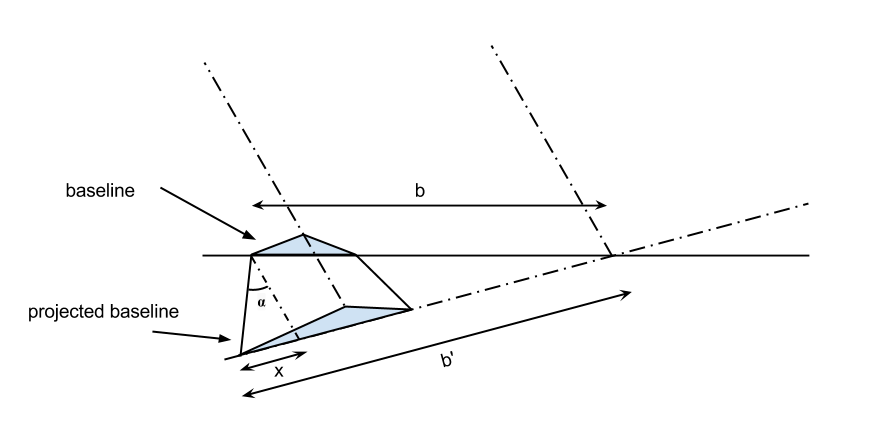
\includegraphics[width=\columnwidth]{W_projection.png}
\caption{A projected baseline with non zero pointing.}
\label{fig:proj_base}
\end{figure}
Let $b$ represent the longest baseline, and $b'$ represent the projected baseline. We wish to find the ratio $b'/b$.

By inspection we can see that the projected baseline length can be determined from a pure geometric projection combined with the diffraction opening angle, $\alpha$. Mathematically,
\begin{equation}
b' = b\cos(\theta) + x = b\cos(\theta) + b\sin(\theta)\tan(\alpha).
\end{equation}
Alpha is approximately half of the primary beam width. So our ratio becomes
\begin{equation} \label{eq:bprimeb}
\frac{b'}{b} = \cos(\theta) + \sin(\theta)\tan(\mathrm{FoV}/2)
\end{equation}
We can plot this ratio as a function of $\theta$ for a conservative field of view of 40$^{\circ}$ (Fig. \ref{fig:bprimeb}).
\begin{figure}[h!] 
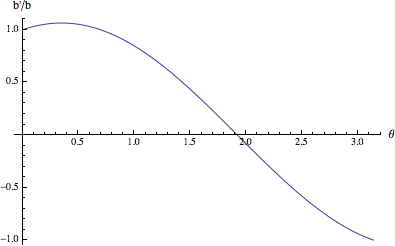
\includegraphics[width=\columnwidth]{bprimeb.png}
\caption{Projected baseline ratio as a function of pointing angle.}
\label{fig:bprimeb}
\end{figure}

We are mostly interested in the maximum of this ratio. We set the derivative with respect to theta equal to zero and solve.
\begin{subequations}
\begin{align}
\frac{\partial}{\partial\theta}(b'/b)  = -\sin(\theta) + \cos(\theta)\tan(\mathrm{FoV}/2) &= 0 \\
 \tan(\theta_{max}) & = \tan(\mathrm{FoV}/2) \\
 \rightarrow \theta_{max} &= \mathrm{FoV}/2
\end{align}
\end{subequations}
Plugging this result back into Eq. \ref{eq:bprimeb}, we have the maximum ratio for a given field of view.
\begin{subequations}
\begin{align}
\left.\frac{b'}{b}\right\vert_{\theta_{max}} & = \cos(\mathrm{FoV}/2) + \sin(\mathrm{FoV}/2)\tan(\mathrm{FoV}/2) \\
& = \sec(\mathrm{FoV}/2)
\end{align}
\end{subequations}


\end{document}